\subsection{Injection-Schwachstellen}

Zur dieser Schwachstellenkategorie zählen typischerweise SQL-, LDAP-, 
OS-Command oder XPath-Injections. Diese Schwachstellen treten bei 
Anwendungen auf, die nicht vertrauenswürdige Eingaben 
(z.B. Eingaben durch einen Anwender) unzureichend prüfen.


\subsubsection{SQL-Injection-Schwachstellen}

Die SQL-Injection-Technik wurde 1998 im Phrack Magazin \cite{rfp_nt_1998}
%\footnote{\url{http://www.phrack.org/issues.html?issue=54\&id=8\#article}} 
einem breiten Publikum vorstellt. Mithilfe einer SQL-Injection-Schwachstelle 
kann ein Angreifer über einen serverseitig unzureichend 
validierten Eingabeparameter beliebige Datenbankbefehle an eine der 
Webanwendung nachgelagerte Backend-Datenbank senden.

Alle gängigen Programmiersprachen sind – unabhängig von den folgenden 
Beispielen – für SQL-Injections anfällig. Dabei sind Runtime-basierende 
Sprachen, wie beispielsweise Java oder C\#, aufgrund ihrer  restriktiven 
Typprüfung tendenziell weniger anfällig für diese Art von Schwachstelle 
als klassische Scriptsprachen wie PHP oder Perl.
\\
\mbox{}
\textbf{Beispiel}
\\
Eine Applikation verfügt über eine Suchfunktion, die es einem Anwender 
ermöglicht, über ein Suchformular nach Benutzer-IDs zu suchen. 
Die Suche ist über das Suchformular "suche.php" realisiert.
\\
\mbox{}
\textbf{Regulärer Aufruf der Anwendung:}
\mbox{}
\\
\textbf{URL:} \texttt{http://www.beliebigedomain.de/suche.php?id=4711}
\\
\textbf{Erzeugtes SQL-Statement:}
\begin{lstlisting}[basicstyle=\ttfamily\footnotesize]
SELECT benutzer, email FROM users WHERE id=4711;
\end{lstlisting}
Da die Anwendung den Wert des Übergabeparameters "id" nicht ausreichend validiert, kann ein Angreifer das SQL-Statement beliebig erweitern:
\\
\textbf{Aufruf der Anwendung mit URL angehängtem, encodierten SQL-Statement}
\\
\textbf{URL:} \texttt{http://www.beliebigedomain.de/suche.php?id=4711\%3B\%20UPDATE\%20users\\\%20SET\%20isAdmin\%3D1\%20WHERE\%20id\%3D235\%3B}
\\
\textbf{Erzeugtes SQL-Statement:}
\begin{lstlisting}[basicstyle=\ttfamily\footnotesize]
SELECT benutzer, email FROM users WHERE id=4711; 
UPDATE users SET isAdmin=1 WHERE id=235;
\end{lstlisting}


Um potenzielle SQL-Injection-Schwachstellen innerhalb einer Anwendung 
zu finden, existieren eine Vielzahl von kommerziellen Anwendungen 
(z.B. Havij\footnote{\url{http://www.itsecteam.com/products/havij-v116-advanced-sql-injection/}}) 
als auch Open-Source-Tools (z.B. Sqlmap\footnote{\url{http://sqlmap.org/}}).

\newpage
\minisec{Sqlmap}

Bei Sqlmap handelt es sich um ein Open-Source-Tool, um SQL-Injection-Schwachstellen 
automatisiert zu finden und auszunutzen. Bei Sqlmap 
handelt es sich um eine konsolenbasierte Anwendung. Das kommerzielle 
Tool Havij bietet dem Anwender hingegen eine grafische Menüführung an.

Im folgenden Beispiel besteht die Vermutung, dass einer der folgenden 
POST-Parameter für SQL-Injection anfällig ist. Dabei ist im Vorfeld der 
Überprüfung bekannt, dass es sich bei der Backend-Datenbank um eine 
MSSQL-Datenbank handelt. Um dies automatisiert zu verifizieren, wird 
Sqlmap mit folgenden Parametern aufgerufen:

\begin{lstlisting}[basicstyle=\ttfamily\footnotesize]
sqlmap.py -u "http://www.beispiel.de"
--data="p1=index.aspx?txtMail=user@name.de&txtPw=geheim&cmdSend=Login" 
--dbms=mssql --risk=3 --level=3
\end{lstlisting}

Ist einer der Parameter für SQL-Injection-Angriffe anfällig, werden 
Informationen zum darunterliegen Betriebssystem, der eingesetzten 
Datenbank sowie Details zur der verwendeten Injection-Technik 
ausgegeben.

\begin{lstlisting}[basicstyle=\ttfamily\footnotesize]
[INFO] the back-end DBMS is Microsoft SQL Server
web server operating system: Windows Vista
web application technology: ASP.NET, ASP, Microsoft IIS 7.0
back-end DBMS: Microsoft SQL Server 2008

Place: POST
  Type: AND/OR time-based blind
  Title: Microsoft SQL Server/Sybase time-based blind
  Payload: p1=index.aspx?txtMail=user@name.de' WAITFOR DELAY '0:0:5'
  --&txtPw=geheim&cmdSend=Login
\end{lstlisting}

Wie der Ausgabe zu entnehmen ist, wird als Datenbanksystem das Microsoft 
Produkt SQL-Server 2008 auf einem Microsoft Windows Vista betrieben. 
Der Parameter \texttt{txtMail} ist für einen time-based blind 
SQL-Injection-Angriff anfällig.

\minisec{Time-based blind SQL-Injection}

Bei einer "Blind SQL-Injection" geht aus den Fehlermeldungen des 
Datenbanksystems nicht hervor, ob eine Anfrage an die Datenbank 
erfolgreich war oder nicht. Durch die Korrelation von verschiedenen 
Details, wie z.B. provozierte Veränderungen der Laufzeiten durch 
einen Angreifer oder kleinste Änderungen innerhalb der 
DBMS-Fehlermeldung können Rückschlüsse auf den Erfolg einer Anfrage 
gezogen werden.
 
Um beispielsweise den Namen der Datenbank mit Hilfe einer 
"time-based blind" SQL-Injection herauszufinden bzw. zu erraten 
(enumerieren) wird im verwendeten Beispiel für jeden richtig geratenen 
Buchstaben der gesuchten Datenbank-Bezeichnung eine Pause von 5 Sekunden 
eingelegt. Auf diese Weise kann ein Angreifer feststellen, ob eine 
Datenbankanfrage erfolgreich war oder nicht bzw., ob der übergebene 
Buchstabe ein Teil der Datenbank-Bezeichnung war. 

Die Enumeration ist jedoch nicht ausschließlich auf den Datenbanknamen 
oder die Datenbanktabellen begrenzt, ebenso kann der aktuelle 
Datenbankbenutzer enumeriert werden oder sogar Betriebssystembefehle 
über diese Schwachstelle abgesetzt werden.

Für weitere Hintergrundinformationen zu den einzelnen 
SQL-Injection-Techniken wird auf das SQL-Injection-Cheat-Sheet
\footnote{\url{http://ferruh.mavituna.com/sql-injection-cheatsheet-oku}} 
verwiesen.

\subsubsection{OS-Command-Injection}

OS-Command-Injection-Schwachstellen verhalten sich sehr ähnlich zu 
SQL-Injection-Schwachstellen. Dabei werden beispielsweise über eine 
Webanwendung Betriebssystembefehle eingeschleust und ausgeführt.
\\
\textbf{Beispiel-1:} Regulärer Aufruf eines Perl CGI-Scripts zur Ausgabe von aktuell am System angemeldeten Benutzern
\\
\textbf{URL:} \texttt{http://www.beliebigedomain.de/showUser.cgi?username=randomUser}
\\
\textbf{Erzeuger Perl-CGI-Code:}
\\
\texttt{\footnotesize{print `who | grep \$username`;}}
\\
\textbf{Beispiel-2:} Aufruf des CGI-Scripts mit angehängten Betriebssystembefehlen
\\
\textbf{URL:} \texttt{http://www.beliebigedomain.de/showUser.cgi?\\username=randomUser;ls\%20-la}
\\
\textbf{Erzeuger Perl-CGI-Code:}
\\
\texttt{\footnotesize{print `who | grep \$username; ls -la`;}}
\\
Durch ein Anhängen des \texttt{ls}-Befehls an den GET-Parameter 
\texttt{username} wird nicht nur nach dem übergebenen Benutzernamen 
innerhalb der \texttt{who}-Ausgabe gesucht, sondern auch der Inhalt 
des aktuellen Verzeichnisses ausgegeben.

\subsection{Maßnahmen zur Behebung von Injection-Schwachstellen}

Um Anwendungen vor Injection-Schwachstellen zu schützen, empfiehlt es 
sich generell, neben einer serverseitigen Validierung aller 
Eingabeparameter und deren Prüfung auf kritische Zeichenketten wie 
beispielsweise Anführungszeichen oder Semikola, bereits im 
Entwicklungsprozess regelmäßig eine statische Quellcode-Analysen 
durchzuführen.

\subsubsection{Maßnahmen zur Behebung SQL-Injection-Schwachstellen}
In diesem Abschnitt werden mögliche Maßnahmen zur Behebung von 
SQL-Injection-Schwachstellen vorgestellt.
\newpage
\minisec{Escapen von Metazeichen}\label{escpace_metazeichen}

Werden Strings für Datenbankabfragen dynamisch generiert, dürfen dabei 
keine unerwünschten Metazeichen in den String eingebaut werden. Werden 
unerlaubt Metazeichen übergeben, müssen diese erkannt und "entschärft" 
werden.

\begin{lstlisting}[basicstyle=\ttfamily\footnotesize]
function SQLStringReplacement)$s) {
    $s = str_replace("'", "''", $s );
    $s = str_replace("\\", "\\\\", $s );
    [...]
}
\end{lstlisting}


Mit obigem Beispielquelltext werden die SQL-Metazeichen "'" und Backslash 
verdoppelt. Diese Verdopplung führt dazu, dass die Metazeichen vom 
Datenbanksystem nicht mehr interpretiert werden. 

An dieser Stelle wird jedoch empfohlen, aufgrund der Fehlerträchtigkeit 
von selbst entwickelten "Escaping"-Lösungen auf verbreitete 
(Framework-)Lösungen wie beispielsweise die OWASP Enterprise 
Security API\footnote{\url{https://www.owasp.org/index.php/Category:OWASP\_Enterprise\_Security\_API}} 
zurückzugreifen.

\minisec{Verwendung von Prepared Statements}

Statt das Escaping der Metazeichen eigenständig oder auf Basis einer 
Framework-Lösung durchzuführen, können auch Prepared Statements verwendet 
werden, um die Injection von unerwünschten Parameterwerten in ein 
SQL-Statement zu verhindern.

\begin{lstlisting}[basicstyle=\ttfamily\footnotesize]
prepStatement string = conn.prepareStatement (
"SELECT benutzer, email FROM users WHERE id=?"
);
\end{lstlisting}

In einem Prepared Statement wird die SQL-Anweisung nicht mehr 
vollständig dynamisch generiert, sondern wird von einem Entwickler 
bis auf die benötigten Parameterwerte bereits im Quelltext vordefiniert. 
In obigem Prepared Statement könnte die Sicherheit noch erhöht werden, 
indem beispielsweise noch geprüft wird, ob es sich bei dem übergebenen 
Parameterwert um einen (erwarteten) Integer-Wert handelt.

\subsubsection{Maßnahmen zur Behebung von OS-Command-Injection}

In diesem Abschnitt werden mögliche Maßnahmen zur Behebung von 
OS-Command-Injection-Schwachstellen vorgestellt.

\minisec{Escapen von Metazeichen}

Identisch mit den Empfehlungen zur Behebung einer SQL-Injection-Schwachstelle, 
allerdings betrifft es hierbei keine Datenbank-Metazeichen sondern die 
Shell-\\Metazeichen.

\newpage
\minisec{Benutzereingaben als Übergabeparameter verhindern}

Um beim Aufruf einer Konsolenanwendung aus einem laufenden Programm 
heraus zu verhindern, dass vom Benutzer beliebiger schadhafter Code zur 
Ausführung kommt, sollte auf die Verwendung vom Anwender wählbarer 
Übergabeparameter vollständig verzichtet werden.

\minisec{Verwendung von Funktionen der Programmiersprache statt Shell-Befehlen}

Im Idealfall wird auf den Aufruf von externen Shell-Programmen aus einem 
laufenden Programm heraus vollständig verzichtet. Stattdessen werden 
native Funktionen der verwendeten Programmiersprache verwendet.


\subsection{Cross-Site-Scripting-Schwachstellen}

Cross-Site-Scripting-Schwachstellen (kurz: XSS) ähneln stark den 
Injection-Schwachstellen. Die Schwachstellen basieren, ähnlich den 
Injection-Schwachstellen, auf einer unzureichenden Eingabevalidierung. 
Bei dieser Schwachstellenkategorie wird HTML- oder JavaScript-Code in den 
Browser des Anwendungsnutzers eingeschleust und dort interpretiert. 
Cross-Site-Scripting-Schwachstellen lassen sich generell in zwei 
Arten unterscheiden:


\subsubsection{Persistentes Cross-Site-Scripting}

Bei persistentem Cross-Site-Scripting wird der applikationsfremde 
JavaScript-Code dauerhaft (z.B. in ein Datenbankfeld) in einer 
webbasierten Anwendung platziert. Besucht ein Nutzer eine betroffene 
Anwendung, in der dieser schadhafte JavaScript-Code eingebettet ist, 
wird der Schadcode ohne weitere Interaktion mit dem Benutzer übertragen 
und in dessen Browser interpretiert bzw. ausgeführt.

\subsubsection{Nicht-persistentes Cross-Site-Scripting}

Bei nicht-persistentem Cross-Site-Scripting (auch reflexives 
Cross-Site-Scripting genannt) muss der JavaScript-Code dagegen mit 
jeder Anfrage an die Anwendung übertragen werden. Dies kann ein 
Angreifer beispielsweise dadurch erreichen, indem er dem Opfer 
eine E-Mail zustellt, die einen Link mit entsprechend präparierten 
Parameterwerten enthält.

\newpage
\minisec{Beispiel für eine Cross-Site-Scripting-Schwachstelle (reflexiv)}

Der folgende Beispielcode gibt den Wert des Parameters \texttt{msg} 
aus (siehe Abbildung \ref{fig:xss_1}):
\\
\textbf{URL:} \texttt{http://domain.de/FUH/msg.php?msg=das+ist+ein+beispiel}

\begin{lstlisting}[basicstyle=\ttfamily\footnotesize]
<html>
<body>
<h1>Beispiel: Ausgabe des GET-Parameters "msg"</h1>
<br>
<?
echo 'String: '. $_GET["msg"];
?>
</body>
</html>
\end{lstlisting}

Da im Beispiel keine serverseitige Validierung des Parameters 
\texttt{msg} vorgenommen wird, ist der Parameter anfällig für 
Cross-Site-Scripting. Wird an die URL aus dem vorhergehenden 
Beispiel JavaScript-Code angehängt, wird der Code vom Browser 
des Anwenders interpretiert und ausgeführt (siehe Abbildung 
\ref{fig:xss_2}).
\\
\textbf{URL:} \texttt{http://domain.de/FUH/msg.php?msg=das+ist+ein+beispiel\\<script>alert('XSS')</script>}

\begin{figure}[htbp]
 \centering
 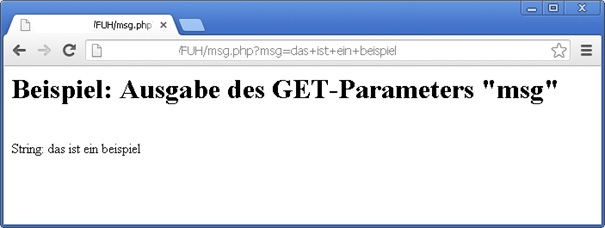
\includegraphics[scale=.75]{abbildungen/xss_1}
 \caption{Ausgabe des Beispiel-Strings}
 \label{fig:xss_1} 
\end{figure}

\begin{figure}[htbp]
 \centering
 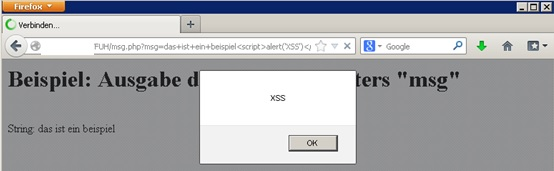
\includegraphics[scale=.75]{abbildungen/xss_2}
 \caption{Der JavaScript-Code kommt im Browser zu Ausführung}
 \label{fig:xss_2} 
\end{figure}

\newpage
Betrachtet man den Quellcode von Abbildung \ref{fig:xss_2}, so 
erkennt man den in HTML eingebetteten JavaScript-Code:

\begin{lstlisting}[basicstyle=\ttfamily\footnotesize]
<html>
  <body>
    <h1>Beispiel: Ausgabe des GET-Parameters "msg"</h1>
    <br>
    String: das ist ein beispiel
    <script>alert('XSS')</script>
  </body>
</html>
\end{lstlisting}

\subsection{Maßnahmen zur Behebung von Cross-Site-Scripting-Schwachstellen}
	
In diesem Abschnitt werden mögliche Maßnahmen zur Behebung von 
Cross-Site-Scripting-Schwachstellen vorgestellt.

\subsubsection{Encoding von HTML-Metazeichen}
	
Durch HTML-Encoding \cite{character_encoding}
%\footnote{\url{http://en.wikipedia.org/wiki/Character\_encodings\_in\_HTML}} 
werden bestimmte HTML-Metazeichen auf äquivalente Zeichenfolgen abgebildet.

Beim Aufruf der URL aus dem Beispiel würde der Wert des Parameters 
\texttt{msg} wie folgt encodiert und im Quelltext dargestellt werden:

\begin{lstlisting}[basicstyle=\ttfamily\footnotesize]
<html>
  <body>
    <h1>Beispiel: Ausgabe des GET-Parameters "msg"</h1>
    <br>
    String: das ist ein beispiel
    &lt;script&gt;alert(&#39;XSS&#39;)&lt;/script&gt;
  </body>
</html>
\end{lstlisting}

Wie der Ausgabe zu entnehmen ist, wurden die typischen HTML-Metazeichen 
serverseitig encodiert und werden aus diesem Grund vom Browser nicht 
mehr als HTML-Metazeichen interpretiert. Der Versuch, eine JavaScript-Messagebox 
mit dem Inhalt "XSS" aufpoppen zu lassen schlug fehl.

\subsubsection{HTML-Tag-Filter}

Bei manchen Systemen (z.B. bei Diskussionsforen) ist ein vollständiges 
HTML-Encoding nicht möglich, da für die Erstellung von Beiträgen 
möglicherweise HTML-Markup benötigt wird. 

Das Vorgehen bei der Verwendung von Tag-Filtern ist ähnlich der 
empfohlenen Maßnahmen zur Behebung von Injection-Schwachstellen 
(siehe Abschnitt \ref{escpace_metazeichen}), bei denen ein Filter auf 
nicht benötigte Zeichen- und Zeichenketten matchen muss. Es ist 
beispielsweise nicht davon auszugehen, dass innerhalb eines 
Diskussionsforums absichtlich ein JavaScript-Tag eingefügt werden 
muss. Aus diesem Grund kann auf den Tag \texttt{<script>} verzichtet 
werden. Ebenso sollte der Filter Schlüsselwörter erkennen, die unter 
Umständen zur Ausführung von JavaScript-Code führen, wie z.B:

\begin{lstlisting}[basicstyle=\ttfamily\footnotesize]
<style type="text/javascript">alert('XSS')</sytle>
\end{lstlisting}

An dieser Stelle sei darauf hingewiesen, dass bei der Verwendung von 
Tag-Filtern (bzw. Blacklist-Filtern) nach Möglichkeit auf eine 
eigenständige Implementierung verzichtet werden und auf 
"Best-Practice"-Lösungen wie beispielsweise die OWASP 
ESAPI-Bibliothek zurückgegriffen werden sollte.

Dabei ist weiterhin zu beachten, dass sich die kritischen HTML-Tags 
zwischen den verschiedenen HTML-Versionen unterscheiden können. 
Durch die Einführung von HTML-5 können beispielsweise Filter, die 
lediglich auf für HTML-4.x relevante Zeichen- und Zeichenketten 
matchen, umgangen werden. Eine ausführliche Beschreibung der 
verschiedensten Umgehungsmöglichkeiten von HTML-4-Filtern durch 
HTML-5-Tags sind im HTML-5-Cheat-Sheet\footnote{\url{http://html5sec.org/}} 
zu finden.

\subsubsection{Verwendung des Model-View-Controller-Pattern}

Im Regelfall benötigt die eigentliche Anwendungslogik keine Details 
über die spätere Darstellung der Informationen. Das bedeutet, dass 
Eingabeparameter auf ihre erwarteten Werte reduziert werden können 
ohne Zusatzinformationen (wie z.B. ihre Darstellung) beinhalten 
zu müssen.

Aus diesem Grund kann man bereits bei der Entwicklung von Anwendungen 
nach dem Model-View-Controler (MVC) Entwicklungspattern vorgehen. Dabei 
werden die Daten (Model), die Darstellung (View) und die 
Benutzerinteraktionen (Controller) strikt voneinander getrennt. 
Benutzereingaben werden auf diese Weise strikt von ihrer späteren 
(erneuten) Darstellung während der Ausgabe getrennt.

Wird dieses MVC-Konzept konsequent bei der Anwendungsentwicklung 
fortgeführt, reduziert sich das Risiko von Cross-Site-Scripting-Schwachstellen 
aufgrund der konsequenten Trennung von Daten und deren Darstellung.

